\documentclass[a4 paper]{article}
\usepackage[inner=2.0cm,outer=2.0cm,top=2.5cm,bottom=2.5cm]{geometry}
\usepackage{setspace}
\usepackage[ruled]{algorithm2e}
\usepackage[rgb]{xcolor}
\usepackage{verbatim}
\usepackage{subcaption}
\usepackage{amsgen,amsmath,amstext,amsbsy,amsopn,tikz,amssymb}
\usepackage{fancyhdr}
\usepackage[colorlinks=true, urlcolor=blue,  linkcolor=blue, citecolor=blue]{hyperref}
\usepackage[colorinlistoftodos]{todonotes}
\usepackage{rotating}
\usepackage{booktabs}
\usepackage{listings}
\usepackage{graphicx}
\newcommand{\ra}[1]{\renewcommand{\arraystretch}{#1}}

\newtheorem{thm}{Theorem}[section]
\newtheorem{prop}[thm]{Proposition}
\newtheorem{lem}[thm]{Lemma}
\newtheorem{cor}[thm]{Corollary}
\newtheorem{defn}[thm]{Definition}
\newtheorem{rem}[thm]{Remark}
\numberwithin{equation}{section}

\newcommand{\homework}[6]{
	\pagestyle{myheadings}
	\thispagestyle{plain}
	\newpage
	\setcounter{page}{1}
	\noindent
	\begin{center}
		\framebox{
			\vbox{\vspace{2mm}
				\hbox to 6.28in { {\bf MATH 118:~Statistics and Probability \hfill {\small (#2)}} }
				\vspace{6mm}
				\hbox to 6.28in { {\Large \hfill #1  \hfill} }
				\vspace{6mm}
				\hbox to 6.28in { {\it Instructor: {\rm #3} \hfill Name: {\rm #5} \hfill Student Id: {\rm #6}} \hfill}
				\hbox to 6.28in { {\it Assistant: #4  \hfill #6}}
				\vspace{2mm}}
		}
	\end{center}
	\markboth{#5 -- #1}{#5 -- #1}
	\vspace*{4mm}
}

\newcommand{\problem}[2]{~\\\fbox{\textbf{Problem #1}}\hfill (#2 points)\newline\newline}
\newcommand{\subproblem}[1]{~\newline\textbf{(#1)}}
\newcommand{\D}{\mathcal{D}}
\newcommand{\Hy}{\mathcal{H}}
\newcommand{\VS}{\textrm{VS}}
\newcommand{\solution}{~\newline\textbf{\textit{(Solution)}} }

\newcommand{\bbF}{\mathbb{F}}
\newcommand{\bbX}{\mathbb{X}}
\newcommand{\bI}{\mathbf{I}}
\newcommand{\bX}{\mathbf{X}}
\newcommand{\bY}{\mathbf{Y}}
\newcommand{\bepsilon}{\boldsymbol{\epsilon}}
\newcommand{\balpha}{\boldsymbol{\alpha}}
\newcommand{\bbeta}{\boldsymbol{\beta}}
\newcommand{\0}{\mathbf{0}}


\begin{document}
	\homework{Homework \#2}{Due: 07/06/21}{Dr. Zafeirakis Zafeirakopoulos}{Gizem S\"ung\"u}{Muhammet Fikret ATAR}{1801042693}
	\textbf{Course Policy}: Read all the instructions below carefully before you start working on the assignment, and before you make a submission.
	\begin{itemize}
		\item It is not a group homework. Do not share your answers to anyone in any circumstance. Any cheating means at least -100 for both sides. 
		\item Do not take any information from Internet.
		\item No late homework will be accepted. 
		\item For any questions about the homework, send an email to gizemsungu@gtu.edu.tr.
		\item Submit your homework (both your latex and pdf files in a zip file) into the course page of Moodle.
		\item Save your latex, pdf and zip files as "Name\_Surname\_StudentId".\{tex, pdf, zip\}.
		\item The answer which has only calculations without any formula and any explanation will get zero. 
		\item The deadline of the homework is 07/06/20 23:55.
		\item I strongly suggest you to write your homework on \LaTeX. However, hand-written paper is still accepted \textbf{IFF} your hand writing is \textbf{clear and understandable to read}, and the paper is well-organized. Otherwise, I cannot grade your homework.
		\item You do not need to write your Student Id on the page above. I am checking your ID from the file name.
	\end{itemize}
	
	\problem{1:}{10+10+10+10+10+10+40 = 100}
	\textbf{WARNING:} Please show your OWN work. Any cheating can be easily detected and will not be graded.
	\newline
	\newline
	For the question, please follow the file called manufacturing\_defects.txt while reading the text below.\\
	\newline
	In each year from 2000 to 2019, the number of manufacturing defects in auto manufacturers were counted. The data was collected from 14 different auto manufactory companies. The numbers of defects for the companies are indicated in 14 columns following the year column. Assume that the number of manufacturing defects per auto company per year is a random variable having a Poisson($\lambda$) and that the number of defects in different companies or in different years are independent.\\
	(Note: You should implement a code for your calculations for each following subproblem. You are free to use any programming languages (Python, R, C, C++, Java) and their related library.)
	
	\subproblem{a} Give a table how many cases occur for all companies between 2000 and 2019 for each number of defects (\# of Defects).\\
	Hint: When you check the file you will see: \# of Defects = \{0, 1, 2, 3, 4\}.\\
	\begin{table}[htb!]
		\centering
		\begin{tabular}{c|c}
			\begin{tabular}[c]{@{}c@{}}\textbackslash{}\# of\\Defects\end{tabular} & \begin{tabular}[c]{@{}c@{}}\textbackslash{}\# of cases\\in all company \\between the years\end{tabular}  \\ 
			\hline
			0                                                                      &                                                                                                 144         \\
			1                                                                      &                                                                                                 91         \\
			2                                                                      &                                                                                                 32        \\
			3                                                          & 11
			\\
			4                                                                      &                                                                                                2        
		\end{tabular}
		
		\caption{Actual cases}
		\label{tab1}
	\end{table}
	
	\subproblem{b} Estimate $\lambda$ from the given data. \\
	$\lambda$ = 0.7 \\
	\subproblem{c} Update Table \ref{tab1} in Table \ref{tab2} with Poisson predicted cases with the estimated $\lambda$.\\
	\begin{table}[htb!]
		\centering
		\begin{tabular}{c|c|c}
			\begin{tabular}[c]{@{}c@{}}\textbackslash{}\# of\\Defects\end{tabular} & \begin{tabular}[c]{@{}c@{}}\textbackslash{}\# of cases\\in all companies\\between the years\end{tabular} & \begin{tabular}[c]{@{}c@{}}Predicted \textbackslash{}\# of cases\\in all companies\\between the years\end{tabular}  \\ 
			\hline
			0                                                                      &                                                                                 144                         &      139.043885                                                                                                               \\
			1                                                                      &                                                                                    91                      &      97.330720                                                                                                               \\
			2                                                                      &                                                                                    32                      &        34.065752                                                                                                             \\
			3                                                                      &                                                                                    11                      &    7.948675
			\\
			4                                                                      &                                                                                       2                   &          1.391018                                                                                                        
		\end{tabular}
		\caption{Actual vs. Predicted Cases}
		\label{tab2}
	\end{table}
	\subproblem{d} Draw a barplot for the actual cases (Table \ref{tab2} in column 2) and the predicted cases (Table \ref{tab2} column 3) with respect to \# of defects. You should put the figure.\\
	

	\centering
	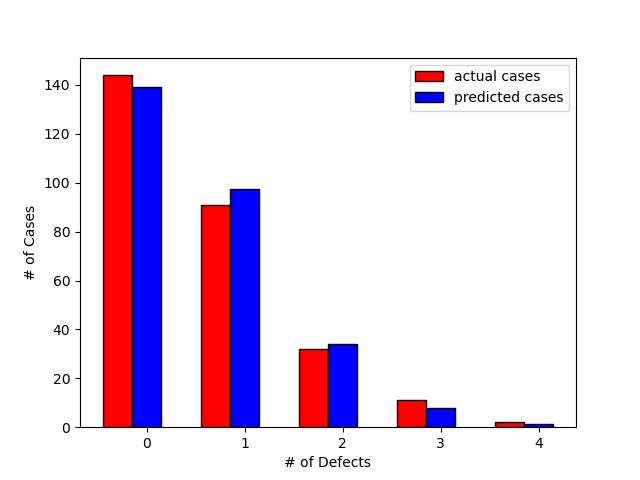
\includegraphics{Figure_1.png}

	
	\subproblem{e} According to the barplot in (c), does the poisson distribution fit the data well? Compare the values of the actual cases and the values of the poisson predicted cases, and write your opinions about performance of the distribution.\\
	When we look at the difference between the actual values and the predicted values, I don't see much difference therefore in my opinion this stuation will not create a big problem,we can say that the distribution fits. The resulting distribution data is suitable.
	The differences are :
4.956115, -6.330719, -2.065752, 0.608981

	\subproblem{f} According to your estimations above, write your opinions considering your barplot and Table \ref{tab2}. Do you think that road transportation is dangerous for us?? Why?\\
	According to our data there are a lot of companies that make good cars with less than 1 defect.Therefore there wouldn’t be a problem in road transportation.In some cases there are few defected cars but number of defected cars are only a few and possibility of a car being defected is so low so we can tolerate the risk of road transportation.As a result in my opinion cosidering my barplot, road transportation is not  dangerous for us.
	\subproblem{g} Paste your code that you implemented for the subproblems above. Do not forget to write comments on your code.\\
	Example:\\
	\begin{itemize}
		\item The common code block for all subproblems\\
		\begin{lstlisting}
import pandas as pd
import numpy as np
import math
import matplotlib.pyplot as plt
from IPython.display import display
data = pd.read_csv('manufacturing_defects.txt', sep='\t', header = None)
#assign some  head this text 
data.columns =['order', 'years','1','2',
              '3','4','5','6',
              '7','8','9','10',
              '11','12','13','14']
#poisson predicted calculate fuction
def Poisson_predicted(number,lamda,totalnumber):
   return (math.exp(-lamda) * (lamda ** number) * totalnumber / math.factorial(number))              
\end{lstlisting}
\end{itemize}
	\begin{itemize}
		\item The code block for (a) \\
		\begin{lstlisting}
print("\nA-)\n")
##remove the some headers
##zeronumbers=(data['1']==0).sum()
data = data.drop(columns="order")
data_edited = data.drop("years", axis=1)
total_zeros=(data_edited.values == 0).sum()
total_one=(data_edited.values == 1).sum()
total_two=(data_edited.values == 2).sum()
total_three=(data_edited.values == 3).sum()
total_four=(data_edited.values == 4).sum()

#print result of numbers of defects

data = {'\# ofDefects':['0', '1', '2', '3','4'], '\# of cases in all company between 
the years':[total_zeros, total_one, total_two, total_three,total_four]}  

#create df for A 
dataframeforA = pd.DataFrame(data) 
#print problem a table
print( dataframeforA.to_string(index=False))
 \end{lstlisting}
\end{itemize}
	\begin{itemize}
		\item The code block for (b)\\
		\begin{lstlisting}
	#problem b solution
	print("B-)Estimate λ from the given data")
	#total value is total defects
	total_value=data_edited.count().sum()
	#total value of defects
	sum_of_values=(total_one*1)+(total_two*2)+(total_three*3)+(total_four*4)
	#estimate λ from the given data
	ave=sum_of_values/total_value
	#print problem b λ
	print("λ-",ave)
 \end{lstlisting}
\end{itemize}
    \begin{itemize}
		\item The code block for (c)\\
		\begin{lstlisting}
#problem c solution
print("\nC-)\nPoisson predicted cases with the estimated λ\n")

#call pp fuction and print result

#create dict for q-)c
data = {'\# ofDefects':[0, 1, 2, 3,4], 
        '\# of cases in all company between the years':
        [total_zeros, total_one, total_two, total_three,total_four],
        'Predicted \# of cases in all companies between the years':
        [Poisson_predicted(0,ave,total_value)
        ,Poisson_predicted(1,ave,total_value)
        ,Poisson_predicted(2,ave,total_value),
        Poisson_predicted(3,ave,total_value)
        ,Poisson_predicted(4,ave,total_value)]}
#create df for q-)c  
dataframeforC = pd.DataFrame(data) 
#print problem c solution
print( dataframeforC.to_string(index=False))
\end{lstlisting}
 \end{itemize}   
    \begin{itemize}
		\item The code block for (d)\\
		\begin{lstlisting}
#print("\nD-) \n")
#height of \# of cases
arr = dataframeforC['\# of cases in all company between the years'].to_numpy()
#height of \# of Predicted \# of cases
arr2= dataframeforC['Predicted \# of cases in all companies between the years'].to_numpy()
w=0.3 
# The x position of bars
r1 = np.arange(len(arr))
r2 = [x + w for x in r1]

# red bar
plt.bar(r1, arr, width = w, color = 'red', edgecolor = 'black', capsize=15, label='actual cases')
 
# blue bar
plt.bar(r2, arr2, width = w, color = 'blue', edgecolor = 'black', capsize=15, label='predicted cases')
 
#graphic editing operation
plt.xticks([r + w for r in range(len(arr))], ['0', '1', '2','3','4'])
plt.ylabel('# of Cases')
plt.xlabel('# of Defects')
plt.legend()
 
# Show graphic
plt.show()
        \end{lstlisting}
	\end{itemize}
	
	
	
	
\end{document} 


